
\documentclass{llncs}

\usepackage{llncsdoc}

\usepackage{times}            % standard fixed width font
\usepackage{graphicx}
\usepackage{amsmath}
\usepackage{xspace}
\usepackage{footnote}
\usepackage{cite}
\usepackage{amsfonts}
\usepackage{subfig}
%\usepackage{natbib}
\usepackage{hhline}
%\usepackage{multirow}
\usepackage{setspace} 
\usepackage{epsfig}
\usepackage[hyphens]{url}
\usepackage[colorlinks,linkcolor=blue,citecolor=blue,urlcolor=blue]{hyperref}
\usepackage[hyphenbreaks]{breakurl}
\usepackage{booktabs}
%\usepackage[compact]{titlesec}
\usepackage{xcolor}
%\usepackage[algoruled,vlined,ruled,linesnumbered]{algorithm2e}
\usepackage{lipsum}
\usepackage{courier}
\usepackage{listings}
\lstset{
  language=C,
	basicstyle=\footnotesize\ttfamily,breaklines=true
}

%\usepackage[T1]{fontenc}
%\usepackage[scaled=0.78]{DejaVuSansMono}

\clubpenalty=10000      % penalty for creating a club line at end of line.
\widowpenalty=10000     % penalty for creating a widow line at top of page.

% Select one or other if want to see comments.
% \com is sometimes displayed during draft.
\long\def\com#1{}
%\long\def\com#1{{\bf \sc comment: }{\small [#1]}{\bf \sc\ endcomment}\newline}

\long\def\xxx#1{{\color{red}{\bf XXX: }{\small [#1]}}}
\long\def\ruzica#1{{\color{red}{\bf Ruzica: }{\small [#1]}}}
%\long\def\xxx#1{}

% Use this macro to force page breaks where ugly widows/orphans occur;
% be sure to recheck all uses after any significant change to the text!
\def\widowpage{\pagebreak}

% Choose abbreviated or long-version alternatives in paper
%\long\def\abbr#1#2{#1}			% abbreviated version
\long\def\abbr#1#2{#2}			% long version

% Choose abbreviations or long names/titles in bibliography
%\def\bibbrev#1#2{#1}			% short version
%\def\bibbrev#1#2{#2}			% long version
\def\bibbrev#1#2{\abbr{#1}{#2}}		% follow abbr macro

% Abbreviated or full citation lists: \abcite{basic}{others}
\newcommand{\abcite}[2]{\abbr{\cite{#1}}{\cite{#1,#2}}}

% Conference abbreviations: \bibconf[Nth]{SOSP}{Symposium on ...}
\newcommand{\bibconf}[3][]{#1 \bibbrev{#2}{#3 (#2)}}

\newcommand{\ie}{{\em i.e.\xspace}}
\newcommand{\eg}{{\em e.g.\xspace}}

% system related terms
\newcommand{\app}{ConfigC\xspace}

% Fault graph terms

\newcommand{\para}[1]{\smallskip\noindent {\bf #1}}

\begin{document}

\special{papersize=8.5in,11in}
\setlength{\pdfpageheight}{\paperheight}
\setlength{\pdfpagewidth}{\paperwidth}

% Uncomment one of the following two, if you are not going for the 
% traditional copyright transfer agreement.

%\exclusivelicense                % ACM gets exclusive license to publish, 
                                  % you retain copyright

%\permissiontopublish             % ACM gets nonexclusive license to publish
                                  % (paid open-access papers, 
                                  % short abstracts)

%\titlebanner{banner above paper title}        % These are ignored unless
%\preprintfooter{short description of paper}   % 'preprint' option specified.

\title{Probabilistic Automated Language Learning for Configuration Files}

\author{~}
\institute{~}
\maketitle


\section*{Abstract}

System failures resulting from configuration errors 
are major reasons for compromised availability and
reliability of today's software systems.
Although many misconfiguration handling techniques
such as checking, troubleshooting, and repair
have been proposed, 
offering automatic verification for configuration files -- as often  
done for regular programs -- is still an open problem.
This is because software configurations are typically written in
poorly structured and untyped ``languages'', and 
specifying constraints and rules for configuration 
verification is non-trivial in practice.

This paper presents \app, the first automatic verification framework for
general software configurations.
\app verifies a target configuration file $F$ through three steps.
Firstly, \app analyzes a dataset containing many sample configuration 
files belonging to the same system as $F$,
translating these sample files to a
well-structured and probabilistically-typed 
intermediate representation.
Secondly, \app derives rules and constraints by analyzing
this intermediate representation, thus building a
sophisticated language model.
Finally, \app uses the resulting language model to verify $F$.
The \app framework is highly modular, 
does not rely on system source code, and
can be applied to any new configuration file type with minimal user input. 

\app is capable of detecting various errors that cannot
be detected by previous efforts,
including entry ordering errors, fine-grained value correlation errors, 
and missing entry errors. 
We evaluate \app using a real-world dataset with 261 incorrect 
MySQL configuration files,
and \app is able to correctly 
detect errors (previous work failed to
detect) in 217 files.



\section{Introduction and System Overview}
\label{sec:Intro}

Configuration errors are one of the most important root-causes of
modern software system failures~\cite{xu15systems,yin11anempirical}.
In practice, misconfiguration problems may result in security
vulnerabilities, application crashes, severe disruptions in software
functionality, and incorrect program executions%
~\cite{xu15systems,zhang14encore,yuan11context}.  Although several
tools have been proposed to automate configuration error diagnosis
after failures occur~\cite{wang04automatic,attariyan10automating,
su07autobash,whitaker04configuration}, these tools rely on a manual approach
  to understand and detect the failure symptoms. The main reasons for this are:
  1) entries in configuration files are untyped assignments, 2) there
  is no explicit structure policy for the entries in configuration
  files, and 3) there are surprisingly few rules specifying the
  entries' constraints.

We propose an approach to the verification of  
configuration files which is based on learning rules about the language 
model for configuration files. 

\begin{figure}[t] \centering
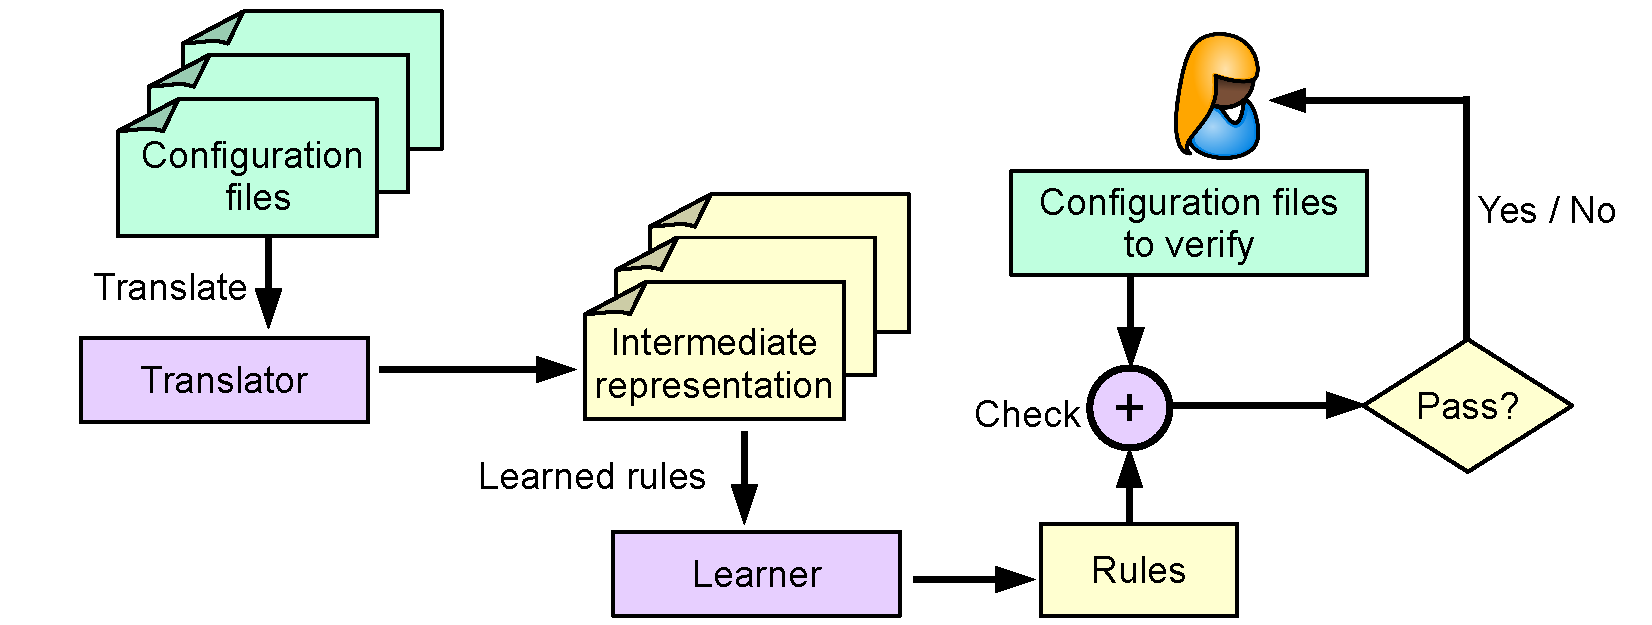
\includegraphics[width=0.65\textwidth]{figs/overview}
\caption{{\footnotesize \app's workflow. The green boxes represent configuration files,
  including both correct general configuration files and users' input
  configuration files. The purple boxes are the components within \app.
  The yellow boxes are results generated by \app's components.}}
\label{fig-overview}
\end{figure}

Figure~\ref{fig-overview} describes an overview of our system. We start
with the assumption that we are given a number of correct configuration
files belonging to the same category (for instance, MySQL or
Apache). Such files follow similar patterns, which we exploit
in a learning algorithm to build rules that
describe a language model for the files. Since the
``language'' of configuration types is untyped and unstructured, we
first parse the files and translate them into a more structured,
intermediary representation.
When running type inference on a configuration file, the type of a variable cannot always be fully determined from a single value.
We address this problem by introducing so called {\emph{probabalistic types}}.
Rather than giving a variable a single type, we assign several types with their probability distributions. 
We can then use these more structured files
as a training set to learn the rules. The learning algorithm
is template-based to be easily extensible. We provide an initial set of templates and the
learner learns some concrete instances from the training set. These
rules are used for detecting errors violating the learned constraints
in the files given by the user.

As an 
illustration of a simple rule that we can learn, consider a template
 $X_1 \le X_2$, where $X_1$ and $X_2$ are
integer variables. The learner might derive the rule stating that
$\texttt{mysql.max\_persistent} \le \texttt{max\_connections}$. There is a classification and taxonomy of configuration errors in the 
existing work on automated configuration troubleshooting~\cite{yin11anempirical, configdataset}. We provide templates for every class that \app can handle: we consider integer constraints, ordering
constraints, typing constraints, and constraints about correlated entries (such as ``if $X$ is present, $Y$ has to appear as well''). 
Unfortunately, we cannot handle the class of errors that rely on the analysis of the whole operating system.
Our language-based approach can only learn on sets of text files, not the system environment.

From a practical perspective \app introduces no additional burden 
to the users: they can simply use \app to check for errors in their configuration files. However, they can also easily extend the framework themselves. The system is designed to be highly modular. If there is a class of rules that \app is not currently learning, the user can develop their own templates and learners for that class. The new learner can be added to \app and this way it can check additionally a new set of errors.

Finally, from a systems perspective this is the first approach that {\emph{proactively}} checks 
 the correctness of configuration files. All previous work
~\cite{xu15systems,zhang14encore,yuan11context, wang04automatic,attariyan10automating,
su07autobash,whitaker04configuration} tries to identify the problem after the
failure occured. Our approach isolates potential errors before the system failure occurs, e.g. before the installation. We can also see \app as a tool that can run in conjunction with existing tools. Pre-analyzed configuration files are already free from language-based errors, and this way the workloads of post-failure forensics at the runtime
is significantly reduced, thus making these tools truly practical.

To summarize, this tool papers makes the following contributions:

\begin{enumerate}

  \item We designed and implemented a tool, \app, that can learn a language model from an example set of correct configuration files, and we use the model to verify new files.
  \item We use probabilistic types to assign a confidence distribution over a set of types to a value.
  \item In \app we define a interface for describing a verification attribute in a learning context, making it easy to add new rules to the system.

\end{enumerate}


\section{Quantum Types}

Because our type inference is based on machine learning, we cannot be sure that a keyword unambigously has a single type.
This is an issue when we try to learn relational rules between keywords. 
Take the following file in the learning

foo = 300
bar = 300.txt


We want to learn the rule that $foo \in {substring(bar)}$, however using unambigous type inference, we would assign foo type int, and never try to generate a string relation rule for these two keywords.
By assigning foo a quantum type (e.g. ${Int <90\%>, String <10\%>}$), we can now generate rules for both types.

At runtime, when the user wants to check a file we update the probabilities one last time then 'collapse' the quantum type to a concrete type.
If the concrete type collapses to a Int, we consider the rules for ints, and vice versa.

This idea is closely related to exstentially quantified types.


\section{Learning strategy}

A primary concern in any machine learning type task is to minimize false negatives and false positives.
In the context of configuration file verification,
  a false positive is when \app reports an error on a valid confiuration file and
  a false negative is when \app fails to reports an error on an invalid confiuration file.
Too many false positives will cause users to ignore the reported error\cite{}.
However, since the cost of system failure is so high from a misconfiguration, \app propritzes the minimization of false negatives.

While a traditional classififcation learning machine learning approach can reduce both of these situations, there is can generally be no garuntee that all false negatives will be eliminated.
Instead of building classification models over the learning set (such as an SVM), we learn the largest set of rules that all correct configuration files satisfy.
In this way, \app can garuntee that, over the set of rules we consider, there will be no false negatives that could have been caught with the given learning set.
The only case of a false negative can be when there was no evidece of such a rule in the learning set - we cannot generate rules from nothing.
Framed as the question "Is this file valid", \app is complete but not sound. 

That is, taking the following definitions:
\begin{multline*}\\
\text{\{Considered Rules\}} = \forall files \in \text{\{Learning Set\}}, \{ r | r(files) = True \land r \text{ is non-trivial}\}\\
\text{\{Reported Rules\}} = {r | r(userfile)=False } \\
\text{\{True Rules\}} = \{r | \text{ if } r(userfile)=False \text{ then system crash } \land \\
   \exists file \in \text{\{Learning Set\}}, r(file) \text{ is non-trivial}\}
\end{multline*}

We have the following specification of \app.
\begin{multline*}\\
\text{\{True Rules\}} \subseteq \text{\{Considered Rules\}} \\
\forall r \in \text{\{True Rules\}}, if r(userfile)=False then \exists r \in \text{\{Reported Rules\}} \\
\neg \forall r \in \text{\{Reported Rules\}}, r \in \text{\{True Rules\}} \\
\end{multline*}

Another benefit to a rule based approach is that, unlike many classificaton models, \app can actually report the reason for failure, similar to a comiler for a programming language.
This is in contrast to neural nets for example, where we would just get a boolean value, and the mechanics of the system are entirly lost.
Reporting useful errors that specify a point of failure is important to help users fix their misconfigurations.

\section{Intermediate Representation}

Part of the reason configuration file errors are so common is because of the large number of different systems being used on the market.
Rather than proposing a new, unifying, configuration language (so that there would then be n+1 configuration languages), we use in intermediate representation language.
This allows us to reuse all our algorithms over any configuration file that can be convereted to the intermediate representation.
The portability of \app means that with very little intervtion, it can be widely used and adopted.

More grammatically complex languages tend to be harder to translation to an intermediate representation.
While there can be some context senestive structures in configuration files, we found it is easier to design the rule modules (Section \ref{}) to handle learning such structure, rather than encoding it in the intermediate representation.
Additionally, configuration files are generally grammatically simple, consisting mostly of a list of keyword-value pairs.
The keyword is the variable to be used in the system, and the value is the new value for that variable.

To specialize the converter for a particular language, a user must define a new language type, which simply acts as a flag for translation.
If a langauge requires specialized parsing, the user can write such code in the convert function based on pattern matching over the language type.
For example, the user must specify the delimiters of the language (characters for assignment and comments) for their new language. 

\section{Rules}

A core design principle in \app is modularity, so that a user can easily exentend it to their verification needs.
Rather than try to support every type of verification over configuration files, we provide a framework for defining new verfication properties.
We call each verification property a rule, for example the correct ordering of keywords or integer relationships between values.
These rules tend to be pairs of values with a relation.
For instance, an integer relation rule might be that the value of "foo" must be greater than the value of "bar".
It is also important that the rule has some empty value, to state that it is known there is no relation between the values.
This will prevent \app from trying to relearn rules when they have already been refuted.

These rules are represented as a type, where the type must support a particular interface (called a typeclass in Haskell) to be compatible with our system.
The typeclass can support anything that is Foldable, which roughly the user can use any datastructure.
In fact, in our implementation, two rules are implemented with lists, and two others use hashmaps.

\begin{lstlisting}
class Foldable t => Attribute t a where
  learn :: IRConfigFile -> t a
  merge :: t a -> t a -> t a
  check :: t a -> IRConfigFile -> Error
\end{lstlisting} 

The functions of this typeclass will be used, invisibly to the user, to make the overall system run.
As long as the specifications for each function are met, \app can garuntee completness.

\subsection{learn}
  For a single given file in the intermediate representation format, learn the full set of rules on that file.
  By overfitting to each file, we can eventually garuntee the completness of \app.
  The specification of this function is the obvious reduction of the Considered Set definition.

  $\text{learn } file =  \{ r | r(file) = True \land r \text{ is non-trivial}\}$

\subsection{merge}
  Merging the sets of rules from two files to build a new set that is true over both files is the most difficult and important function a rule must implement.
  This is generally implemented as a filter over the union of the two set, but may vary slightly.
  The formal specification of this method is that:
  \begin{multline*}
  \text{merge } Set1 \: Set2= \{r \mid \\
    r \in \text{Set1} \cup \text{Set2} \land \\
    \exists file \forall r' \in \text{Set1} \cup \text{Set2}, r(file) = True \land r'(file) = True \} \\
  \end{multline*}

\subsection{check}
  To check a file by using a rule set, we simply take all the rules that are releveant to the user's file.
  Rules that are relavent are the ones where both parts of the ordering are present.
  We learn the rule set for the user file, and every rule in the learned set must be present in the user file.

\section{Implementation}

\subsection{System}
Since we learn a set of rules on each file in isolation from the other, we have an embarrassing parallel situation.
Haskell allows us to easily take advantage of by using the parallel mapping library, parmap, both for translation to the intermediate representation, and for learning the rules on each file.
\xxx{merge can also be parallelized, but i haven't done it yet and might not get a chance}

\begin{lstlisting}
learnRules :: [ConfigFile Language] -> RuleSet
learnRules fs = let
  fs' = parMap rseq convert fs
  rs = parMap rdeepseq findAllRules fs'
 in
  foldl1 mergeRules rs
\end{lstlisting}

\subsection{Type Error Rules}
This builds a map between keywords and types, using the values as evidence.
see quantum.tex for more
i will write more on this tomorrow.

\subsection{Integer Relation Rules}
we only consider the relations , (==), (<=), (>=) because they are easy to pass aroud (as actual functions) in haskell.
We also committed cardinal since and create an instance for equality over these functions.
instance Eq (Int->Int->Bool) where

With more engineering effort, this could be extened with the use of a SMT solver to create more fine grained relational rules.
From our experience, more specific rule are not really needed for integer relations in configuration files.
However an SMT solver approach would be particularly useful for relations on strings, especially when considering substring relations between filepaths.

\subsection{Ordering and Missing Entry Rules}
These are the simpiliest of all rules, just making a lot of pairs and seeing which pairs continue to appear over the learning set.

There is actually a bit of a catch in ordering though - we are not complete over ordering rules.
This is because only our implementation does not satisfy the specification for the merge function listed above.
The problem arises from the fact the configuration files may have non-unique keywords.
Therefor, in the follwoing file we will derive the valid, but conflicting rules ([client],port) and (port,[client]).
\begin{verbatim}
[client]
port = 3306
[mysqld]
port = 3306
\end{verbatim}
Our implementation of merge removes and conflicting rules for the running set.
By introducing a renaming pass in the initial parsing we may be able to solve this, but have not found a satisfactory solution yet.

%
\section{Learning strategy}

A primary concern in any machine learning type task is to minimize false negatives and false positives.
In the context of configuration file verification,
  a false positive is when \app reports an error on a valid confiuration file and
  a false negative is when \app fails to reports an error on an invalid confiuration file.
Too many false positives will cause users to ignore the reported error\cite{}.
However, since the cost of system failure is so high from a misconfiguration, \app propritzes the minimization of false negatives.

While a traditional classififcation learning machine learning approach can reduce both of these situations, there is can generally be no garuntee that all false negatives will be eliminated.
Instead of building classification models over the learning set (such as an SVM), we learn the largest set of rules that all correct configuration files satisfy.
In this way, \app can garuntee that, over the set of rules we consider, there will be no false negatives that could have been caught with the given learning set.
The only case of a false negative can be when there was no evidece of such a rule in the learning set - we cannot generate rules from nothing.
Framed as the question "Is this file valid", \app is complete but not sound. 

That is, taking the following definitions:
\begin{multline*}\\
\text{\{Considered Rules\}} = \forall files \in \text{\{Learning Set\}}, \{ r | r(files) = True \land r \text{ is non-trivial}\}\\
\text{\{Reported Rules\}} = {r | r(userfile)=False } \\
\text{\{True Rules\}} = \{r | \text{ if } r(userfile)=False \text{ then system crash } \land \\
   \exists file \in \text{\{Learning Set\}}, r(file) \text{ is non-trivial}\}
\end{multline*}

We have the following specification of \app.
\begin{multline*}\\
\text{\{True Rules\}} \subseteq \text{\{Considered Rules\}} \\
\forall r \in \text{\{True Rules\}}, if r(userfile)=False then \exists r \in \text{\{Reported Rules\}} \\
\neg \forall r \in \text{\{Reported Rules\}}, r \in \text{\{True Rules\}} \\
\end{multline*}

Another benefit to a rule based approach is that, unlike many classificaton models, \app can actually report the reason for failure, similar to a comiler for a programming language.
This is in contrast to neural nets for example, where we would just get a boolean value, and the mechanics of the system are entirly lost.
Reporting useful errors that specify a point of failure is important to help users fix their misconfigurations.

\section{Intermediate Representation}

Part of the reason configuration file errors are so common is because of the large number of different systems being used on the market.
Rather than proposing a new, unifying, configuration language (so that there would then be n+1 configuration languages), we use in intermediate representation language.
This allows us to reuse all our algorithms over any configuration file that can be convereted to the intermediate representation.
The portability of \app means that with very little intervtion, it can be widely used and adopted.

More grammatically complex languages tend to be harder to translation to an intermediate representation.
While there can be some context senestive structures in configuration files, we found it is easier to design the rule modules (Section \ref{}) to handle learning such structure, rather than encoding it in the intermediate representation.
Additionally, configuration files are generally grammatically simple, consisting mostly of a list of keyword-value pairs.
The keyword is the variable to be used in the system, and the value is the new value for that variable.

To specialize the converter for a particular language, a user must define a new language type, which simply acts as a flag for translation.
If a langauge requires specialized parsing, the user can write such code in the convert function based on pattern matching over the language type.
For example, the user must specify the delimiters of the language (characters for assignment and comments) for their new language. 

\section{Rules}

A core design principle in \app is modularity, so that a user can easily exentend it to their verification needs.
Rather than try to support every type of verification over configuration files, we provide a framework for defining new verfication properties.
We call each verification property a rule, for example the correct ordering of keywords or integer relationships between values.
These rules tend to be pairs of values with a relation.
For instance, an integer relation rule might be that the value of "foo" must be greater than the value of "bar".
It is also important that the rule has some empty value, to state that it is known there is no relation between the values.
This will prevent \app from trying to relearn rules when they have already been refuted.

These rules are represented as a type, where the type must support a particular interface (called a typeclass in Haskell) to be compatible with our system.
The typeclass can support anything that is Foldable, which roughly the user can use any datastructure.
In fact, in our implementation, two rules are implemented with lists, and two others use hashmaps.

\begin{lstlisting}
class Foldable t => Attribute t a where
  learn :: IRConfigFile -> t a
  merge :: t a -> t a -> t a
  check :: t a -> IRConfigFile -> Error
\end{lstlisting} 

The functions of this typeclass will be used, invisibly to the user, to make the overall system run.
As long as the specifications for each function are met, \app can garuntee completness.

\subsection{learn}
  For a single given file in the intermediate representation format, learn the full set of rules on that file.
  By overfitting to each file, we can eventually garuntee the completness of \app.
  The specification of this function is the obvious reduction of the Considered Set definition.

  $\text{learn } file =  \{ r | r(file) = True \land r \text{ is non-trivial}\}$

\subsection{merge}
  Merging the sets of rules from two files to build a new set that is true over both files is the most difficult and important function a rule must implement.
  This is generally implemented as a filter over the union of the two set, but may vary slightly.
  The formal specification of this method is that:
  \begin{multline*}
  \text{merge } Set1 \: Set2= \{r \mid \\
    r \in \text{Set1} \cup \text{Set2} \land \\
    \exists file \forall r' \in \text{Set1} \cup \text{Set2}, r(file) = True \land r'(file) = True \} \\
  \end{multline*}

\subsection{check}
  To check a file by using a rule set, we simply take all the rules that are releveant to the user's file.
  Rules that are relavent are the ones where both parts of the ordering are present.
  We learn the rule set for the user file, and every rule in the learned set must be present in the user file.

\section{Implementation}

\subsection{System}
Since we learn a set of rules on each file in isolation from the other, we have an embarrassing parallel situation.
Haskell allows us to easily take advantage of by using the parallel mapping library, parmap, both for translation to the intermediate representation, and for learning the rules on each file.
\xxx{merge can also be parallelized, but i haven't done it yet and might not get a chance}

\begin{lstlisting}
learnRules :: [ConfigFile Language] -> RuleSet
learnRules fs = let
  fs' = parMap rseq convert fs
  rs = parMap rdeepseq findAllRules fs'
 in
  foldl1 mergeRules rs
\end{lstlisting}

\subsection{Type Error Rules}
This builds a map between keywords and types, using the values as evidence.
see quantum.tex for more
i will write more on this tomorrow.

\subsection{Integer Relation Rules}
we only consider the relations , (==), (<=), (>=) because they are easy to pass aroud (as actual functions) in haskell.
We also committed cardinal since and create an instance for equality over these functions.
instance Eq (Int->Int->Bool) where

With more engineering effort, this could be extened with the use of a SMT solver to create more fine grained relational rules.
From our experience, more specific rule are not really needed for integer relations in configuration files.
However an SMT solver approach would be particularly useful for relations on strings, especially when considering substring relations between filepaths.

\subsection{Ordering and Missing Entry Rules}
These are the simpiliest of all rules, just making a lot of pairs and seeing which pairs continue to appear over the learning set.

There is actually a bit of a catch in ordering though - we are not complete over ordering rules.
This is because only our implementation does not satisfy the specification for the merge function listed above.
The problem arises from the fact the configuration files may have non-unique keywords.
Therefor, in the follwoing file we will derive the valid, but conflicting rules ([client],port) and (port,[client]).
\begin{verbatim}
[client]
port = 3306
[mysqld]
port = 3306
\end{verbatim}
Our implementation of merge removes and conflicting rules for the running set.
By introducing a renaming pass in the initial parsing we may be able to solve this, but have not found a satisfactory solution yet.




%
\section{\app Design}

\xxx{
\app Design: 
  \begin{itemize}
  \item Present an architecture of \app with a fig. Briefly describe 
    how it works (step by step).
  \item Detail learner part
  \item Merge
  \item Check 
  \item Limitations
  \end{itemize}
}

\section{Learning strategy}

A primary concern in any machine learning type task is to minimize false negatives and false positives.
In the context of configuration file verification,
  a false positive is when \app reports an error on a valid confiuration file and
  a false negative is when \app fails to reports an error on an invalid confiuration file.
Too many false positives will cause users to ignore the reported error\cite{}.
However, since the cost of system failure is so high from a misconfiguration, \app propritzes the minimization of false negatives.

While a traditional classififcation learning machine learning approach can reduce both of these situations, there is can generally be no garuntee that all false negatives will be eliminated.
Instead of building classification models over the learning set (such as an SVM), we learn the largest set of rules that all correct configuration files satisfy.
In this way, \app can garuntee that, over the set of rules we consider, there will be no false negatives that could have been caught with the given learning set.
The only case of a false negative can be when there was no evidece of such a rule in the learning set - we cannot generate rules from nothing.
Framed as the question "Is this file valid", \app is complete but not sound. 

That is, taking the following definitions:
\begin{multline*}\\
\text{\{Considered Rules\}} = \forall files \in \text{\{Learning Set\}}, \{ r | r(files) = True \land r \text{ is non-trivial}\}\\
\text{\{Reported Rules\}} = {r | r(userfile)=False } \\
\text{\{True Rules\}} = \{r | \text{ if } r(userfile)=False \text{ then system crash } \land \\
   \exists file \in \text{\{Learning Set\}}, r(file) \text{ is non-trivial}\}
\end{multline*}

We have the following specification of \app.
\begin{multline*}\\
\text{\{True Rules\}} \subseteq \text{\{Considered Rules\}} \\
\forall r \in \text{\{True Rules\}}, if r(userfile)=False then \exists r \in \text{\{Reported Rules\}} \\
\neg \forall r \in \text{\{Reported Rules\}}, r \in \text{\{True Rules\}} \\
\end{multline*}

Another benefit to a rule based approach is that, unlike many classificaton models, \app can actually report the reason for failure, similar to a comiler for a programming language.
This is in contrast to neural nets for example, where we would just get a boolean value, and the mechanics of the system are entirly lost.
Reporting useful errors that specify a point of failure is important to help users fix their misconfigurations.

\section{Intermediate Representation}

Part of the reason configuration file errors are so common is because of the large number of different systems being used on the market.
Rather than proposing a new, unifying, configuration language (so that there would then be n+1 configuration languages), we use in intermediate representation language.
This allows us to reuse all our algorithms over any configuration file that can be convereted to the intermediate representation.
The portability of \app means that with very little intervtion, it can be widely used and adopted.

More grammatically complex languages tend to be harder to translation to an intermediate representation.
While there can be some context senestive structures in configuration files, we found it is easier to design the rule modules (Section \ref{}) to handle learning such structure, rather than encoding it in the intermediate representation.
Additionally, configuration files are generally grammatically simple, consisting mostly of a list of keyword-value pairs.
The keyword is the variable to be used in the system, and the value is the new value for that variable.

To specialize the converter for a particular language, a user must define a new language type, which simply acts as a flag for translation.
If a langauge requires specialized parsing, the user can write such code in the convert function based on pattern matching over the language type.
For example, the user must specify the delimiters of the language (characters for assignment and comments) for their new language. 

\section{Rules}

A core design principle in \app is modularity, so that a user can easily exentend it to their verification needs.
Rather than try to support every type of verification over configuration files, we provide a framework for defining new verfication properties.
We call each verification property a rule, for example the correct ordering of keywords or integer relationships between values.
These rules tend to be pairs of values with a relation.
For instance, an integer relation rule might be that the value of "foo" must be greater than the value of "bar".
It is also important that the rule has some empty value, to state that it is known there is no relation between the values.
This will prevent \app from trying to relearn rules when they have already been refuted.

These rules are represented as a type, where the type must support a particular interface (called a typeclass in Haskell) to be compatible with our system.
The typeclass can support anything that is Foldable, which roughly the user can use any datastructure.
In fact, in our implementation, two rules are implemented with lists, and two others use hashmaps.

\begin{lstlisting}
class Foldable t => Attribute t a where
  learn :: IRConfigFile -> t a
  merge :: t a -> t a -> t a
  check :: t a -> IRConfigFile -> Error
\end{lstlisting} 

The functions of this typeclass will be used, invisibly to the user, to make the overall system run.
As long as the specifications for each function are met, \app can garuntee completness.

\subsection{learn}
  For a single given file in the intermediate representation format, learn the full set of rules on that file.
  By overfitting to each file, we can eventually garuntee the completness of \app.
  The specification of this function is the obvious reduction of the Considered Set definition.

  $\text{learn } file =  \{ r | r(file) = True \land r \text{ is non-trivial}\}$

\subsection{merge}
  Merging the sets of rules from two files to build a new set that is true over both files is the most difficult and important function a rule must implement.
  This is generally implemented as a filter over the union of the two set, but may vary slightly.
  The formal specification of this method is that:
  \begin{multline*}
  \text{merge } Set1 \: Set2= \{r \mid \\
    r \in \text{Set1} \cup \text{Set2} \land \\
    \exists file \forall r' \in \text{Set1} \cup \text{Set2}, r(file) = True \land r'(file) = True \} \\
  \end{multline*}

\subsection{check}
  To check a file by using a rule set, we simply take all the rules that are releveant to the user's file.
  Rules that are relavent are the ones where both parts of the ordering are present.
  We learn the rule set for the user file, and every rule in the learned set must be present in the user file.

\section{Implementation}

\subsection{System}
Since we learn a set of rules on each file in isolation from the other, we have an embarrassing parallel situation.
Haskell allows us to easily take advantage of by using the parallel mapping library, parmap, both for translation to the intermediate representation, and for learning the rules on each file.
\xxx{merge can also be parallelized, but i haven't done it yet and might not get a chance}

\begin{lstlisting}
learnRules :: [ConfigFile Language] -> RuleSet
learnRules fs = let
  fs' = parMap rseq convert fs
  rs = parMap rdeepseq findAllRules fs'
 in
  foldl1 mergeRules rs
\end{lstlisting}

\subsection{Type Error Rules}
This builds a map between keywords and types, using the values as evidence.
see quantum.tex for more
i will write more on this tomorrow.

\subsection{Integer Relation Rules}
we only consider the relations , (==), (<=), (>=) because they are easy to pass aroud (as actual functions) in haskell.
We also committed cardinal since and create an instance for equality over these functions.
instance Eq (Int->Int->Bool) where

With more engineering effort, this could be extened with the use of a SMT solver to create more fine grained relational rules.
From our experience, more specific rule are not really needed for integer relations in configuration files.
However an SMT solver approach would be particularly useful for relations on strings, especially when considering substring relations between filepaths.

\subsection{Ordering and Missing Entry Rules}
These are the simpiliest of all rules, just making a lot of pairs and seeing which pairs continue to appear over the learning set.

There is actually a bit of a catch in ordering though - we are not complete over ordering rules.
This is because only our implementation does not satisfy the specification for the merge function listed above.
The problem arises from the fact the configuration files may have non-unique keywords.
Therefor, in the follwoing file we will derive the valid, but conflicting rules ([client],port) and (port,[client]).
\begin{verbatim}
[client]
port = 3306
[mysqld]
port = 3306
\end{verbatim}
Our implementation of merge removes and conflicting rules for the running set.
By introducing a renaming pass in the initial parsing we may be able to solve this, but have not found a satisfactory solution yet.


\section{Motivating Examples}
\label{sec:motiv}

When writing configuration files, users usually take already existing
files and modifies the files, with little knowledge of the system. 
The non-expert user can then easily introduce in errors.
Even worse, the original file may already corrupted and the errors are propagated further. 
Below we show some real worlds examples of the errors commonly found in configuration files.
All these examples are extracted from real-world reports % ~\cite{yin11anempirical, configdataset}.
The deep, domain specific knowledge needed to identify these error manually is strong motivation for a tool such as \app.

\para{Example~1: Ordering Errors.} When configuring PHP to run with the
Apache HTTP Server, the user writes, among others, the following lines:\\
 \texttt{
 \hspace*{3em}extension = mysql.so\\
 \hspace*{3em}...\\
 \hspace*{3em}extension = recode.so}\\
This file caused the Apache server to fail to start due to a segmentation fault error.
When using PHP in Apache, the extension ``mysql.so'' depends on ``recode.so'' and the relative ordering of two of them is crucial. 
\app would inform the user that ``recode.so'' should appear before ``mysql.so'', and return the error:\\
 \texttt{
ORDERING ERROR: Expected "extension"recode.so"\\
   BEFORE "extension""mysql.so"
  }

\para{Example~2: Entry Missing Errors.} If the user wants to use OpenLDAP to enable her directory access
protocol, she needs to use the password policy overlay. This is usually
done through the following entries in the OpenLDAP configuration file:\\
\texttt{
 \hspace*{3em}include schema/ppolicy.schema\\
 \hspace*{3em}overlay ppolicy\\}
When using the password policy overlay in OpenLDAP, we have to first include the related schema.
Leaving out the ``include'' statement will cause the failure of 
this LDAP. Running \app on such a misconfiguration file would return:\\
\texttt{
MISSING KEYWORD ERROR: Expected "overlay""ppolicy"\\ 
in the same file as: "include""schema/ppolicy.schema"}

\para{Example~3: Type Errors.} If the user tries to install MySQL, she first needs to initiate the path for the log information generated by MySQL. 
A user may put the following code in the MySQL configuration file:\\
\texttt{
 \hspace*{3em}general\_log = /var/log/mysql/mysql.log\\}
However, the entry ``general\_log'' should be an integer, not a string.
 In MySQL, there is another entry named ``general\_log\_file'' which is used to specify the log path.  
After \app analyzes this configuration file, it correctly identifies the error:\\
\texttt{
TYPE ERROR: Expected a Int with P=1.0 for "general\_log[mysqld]"
}

\vspace{-10pt}
\para{Example~4: Value Correlation Errors.} When configuring PHP on MySQL, the user may write the following lines of entries in both the PHP and MySQL configuration files:\\
\texttt{
 \hspace*{3em}mysql's config\\
 \hspace*{3em}max\_connections = 300\\
 \hspace*{3em}...\\
 \hspace*{3em}php's config\\
 \hspace*{3em}mysql.max\_persistent = 400\\}
This could cause MySQL to abort with the error information: ``too many connections''.
In this case, the ``mysql.max\_persistent'' in PHP should be no larger than the ``max\_connections'' in MySQL configuration file.
Another rule we have implemented is learning inequality relations between integers.
Running \app on this combined configuration file would return:
\texttt{
INTEGER RELATION ERROR: \\
Expected "max\_connections">="mysql.max\_persistent"}

\com{
\begin{figure}[t] \centering
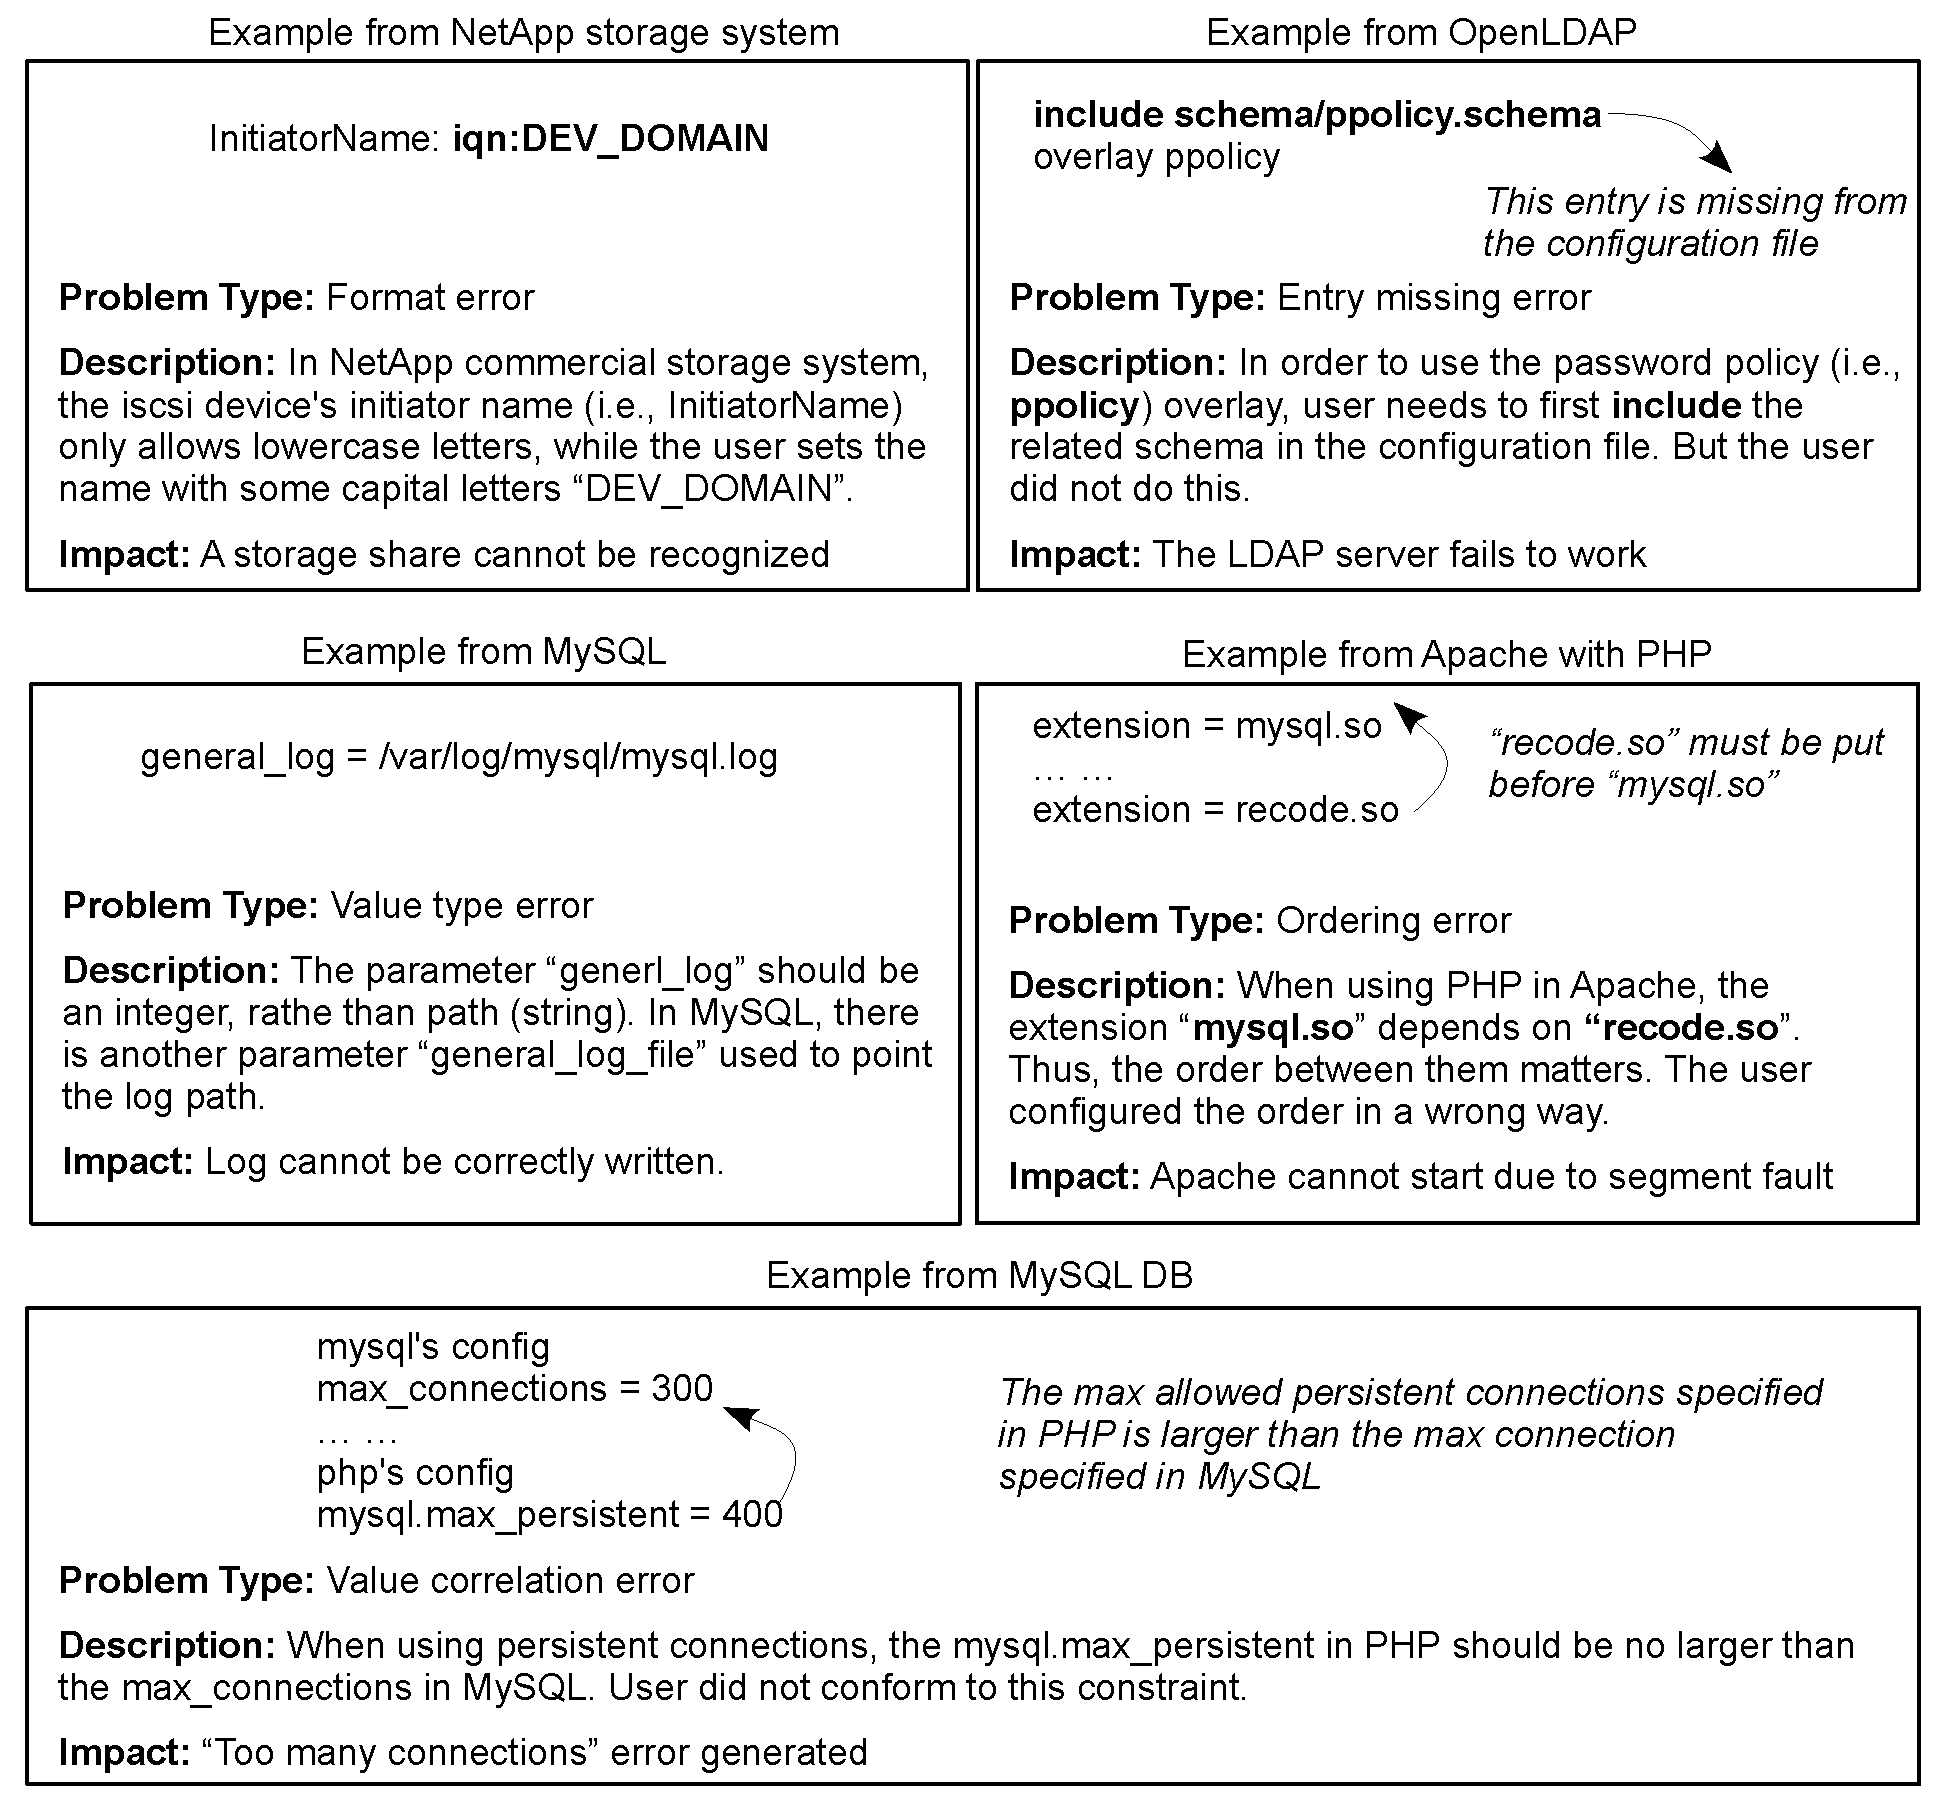
\includegraphics[width=0.98\textwidth]{figs/example}
\caption{Motivating examples. Our target configuration errors are
  classified into five groups. The five examples here correspond to
  these groups, respectively.}
\label{fig-example}
\end{figure}

Fig.~\ref{fig-example} presents misconfiguration examples in real-world
that we aim to address. All the examples are extracted from
misconfiguration issues reported in real-world efforts%
~\cite{yin11anempirical, configdataset}.
We classify our target configuration errors
into five groups: 1) format error; 2) entry missing error; 3) value type
error; and 4) ordering error
The examples in Fig.~\ref{fig-example} correspond to the above four
groups, respectively.

} 

\section{Implementation and Evaluation}

\para{Implementation.}
\app is implemented in Haskell and takes full advantage of its polymorphism to make the system more modular.
In particular, rules are represented as a type, where the type must support a particular interface (called a typeclass in Haskell) to be compatible with our system.
By using language extensions (FlexibleInstances and MultiParamTypeClasses), this typeclass can be made polymorphic over the data structure as denoted by \lstinline{Foldable t =>}.
The user can then choose a data structure that is most natural to the rule they are implementing.
For example, in our implementation, Missing Entries were easier to manipulate in lists, while Type Errors fit more naturally into a hashmap.
This typeclass defines the three functions that each set of rules must implement to work with our system. The core learning algorithm is simply a fold using \lstinline{merge} over the derived rules from running \lstinline{learn} on each file in the learning set.

Typeclasses and other features of Haskell means that our system consists of only 267 lines of code, with another 233 for the rule modules.
With an average size of 58 lines of code for each rule module, this is evidence of how simple it is to extend \app with new rules.

\begin{lstlisting}
class Foldable t => RuleSet t a where
  learn :: IRConfigFile -> t a
  merge :: t a -> t a -> t a
  check :: t a -> IRConfigFile -> Error
\end{lstlisting}

Since we learn a set of rules on each file in isolation from the other, we have a pleasingly parallel situation.
Haskell allows us to easily take advantage of this by using the parallel
mapping library \cite{parallel}, both for translation to the intermediate representation, and for learning the rules on each file.
The merge stage could also easily be parallelized, using a divide and conquer approach, but \app runs fast enough over our learning set (28 files, 961 lines of code) that this has not been necessary.

The integer relation rule has an unusual implementation that uses function as first-class objects in Haskell.
Rather than associated keywords with SMT formula, we directly associate them with a function of type (\lstinline{Int->Int->Bool}).
Since we need to compare rules over equality, we must have a way to compare functions.
This limits the types of functions we use to \lstinline{(==),(>=),(<=)}.
Although this is sufficient for most cases, more fine-grained relations could be encoded with SMT formulas then passed to a solver.

The tool is available for download at \url{http://marksantolucito.com/cavae.html}.


\para{Evaluation.}
To evaluate our tool, we take a subset of 20 benchmarks from an
existing dataset of configuration errors~\cite{yin11anempirical,xu15hey,configdataset} which are supported by our tool. Table~\ref{table:res} contains an evaluation summary.
We do not report the running times, since they are negligible: even when
 running in the interpreter mode, files are analyzed instantaneously. We
spent approximately 30 second on learning the rules. When we run the
compiled version, we need for learning and verification 
combined less than 5 seconds. Our focus is usefulness of the tool: its 
 ability to detect configuration errors and the number of false positives.
 For every benchmark class we took five examples. The middle column represents the number of detected errors, while the right column represents the number of returned false positives per each benchmark.
 


\iffalse{
We take the subset of benchmarks for which our tool has implemented rule modules.
Although our tool is general and extensible, we have only implemented four types of rules over the MySQL configuration language.
It would not make sense to run \app on misconfigurations for which there are no rule modules.}
\fi

A benchmark passes a test if it reports an error on the source of the misconfiguration (it is not a false negative).
We call false positives any reported error that was unrelated to the value of interest.
It is worth noting that this is in fact a conservative estimate.
Since these benchmarks are taken from online forums, there is no guarantee the files contain only a single error.
Indeed, on some benchmarks, \app found errors in the file that were similar to rules broken by other benchmarks. 

We fail one benchmark in Value Relations because we do not yet support relations between file sizes of different units (Mb to Kb).
In one Keyword Ordering benchmark, \app reports a type error on the value of interest instead of an ordering error.
This is a result of our context embedding in the translation to the intermediate representation - reordering the value puts it in a new context where the type is now also incorrect.

\begin{table}[t]
\centering
\caption{Benchmarks for misconfiguration detection}
\label{table:res}
\begin{tabular}{|l|l|l|}
\hline
Error Type       & Passing Tests & False Positives  \\ 
\hline
\hline
Missing Entry    & 5/5           & 1, 0, 0, 0, 4        \\ \hline
Type Error       & 5/5           & 0, 0, 0, 0, 0          \\ \hline
Keyword Ordering & 5/5           & 0, 2, 1, 0, 6       \\ \hline
Value Relations  & 4/5           & 0, 0, 0, 1, 0        \\ 
\hline
\end{tabular}
\end{table}

All but one false positive reports were integer relations. They are the
result of overfitting on rules.
\app can learn overapproximating rules when the learning set does not show the full spectrum of possible values.
Since integer relations have a larger space of relation than ordering relations for instance, \app needs a larger learning set in order to eliminate false positives.

The false positive for the Value Relation was a Missing Entry error.
This is a result of the fact that we cannot learn rules that are disjunctions.
In this case, no socket is provided to [mysqld], failing a rule we had learned over the dataset.
In fact, this is not a misconfiguration because a socket only needs to be provided to one (or both) [mysqld] or [wampsqld].
We reported an error since none of the files in the learning set had no socket associated with [mysqld].
In fact, since we do not support disjunctive rules, we could not have even learned such a rule - though in practice these seem to be uncommon.



\section{Related Work}

\iffalse
Configuration verification has been considered a promising way  
to tackle misconfiguration problems~\cite{xu15systems}.
Nevertheless, a practical and automatic configuration
verification approach still remains an open problem.

\para{Language-support misconfiguration checking}
There have been several language-support efforts proposed for preventing
configuration errors introduced by fundamental deficiencies in
either untyped or low-level languages. For example, in the network
configuration management area, administrators often
produce configuration errors in their routing configuration files.
PRESTO~\cite{enck07configuration} 
automates the generation of device-native configurations
with configlets in a template language. 
Loo {\em et al.}~\cite{loo05declarative} adopt Datalog to reason about 
routing protocols in a declarative fashion. 
COOLAID~\cite{chen10declarative} constructs
a language to describe domain knowledge about devices and
services for convenient network reasoning and management.
Compared with the above efforts, our work focuses on software systems, 
\eg, MySQL and Apache, and our main purpose is to automate configuration
verification rather than proposing new languages 
to convenient configuration-file writing. 

\para{Misconfiguration detection}
Misconfiguration detection techniques aim at checking configuration
efforts before system outages occur.
Most existing detection approaches check 
the configuration files against a set of predefined correctness 
rules, named constraints, and then report errors if 
the checked configuration files do not satisfy these rules.
Huang {\em et al.}~\cite{huang15confvalley},
for example, proposed a 
language, ConfValley, to validate 
whether given configuration files meet administrators' specifications. 
As opposed to our work, ConfValley does not
have inherent misconfiguration checking capability, since it only offers
a language representation and requires administrators to
manually write specifications, which is an error-prone
process. On the contrary, our work does not need users to manually
write anything.

Several machine learning-based misconfiguration detection efforts 
also have been proposed~\cite{yuan11context, zhang14encore, xu16early}.
EnCore~\cite{zhang14encore} introduces a template-based
learning approach to improve the accuracy of their learning results.
The learning process is guided by a set of predefined rule templates
that enforce learning to focus on patterns of interest.
In this way, EnCore filters out irrelevant information and reduces
false positives; moreover, the templates are able to express
system environment information that other machine learning
techniques cannot handle.
Compared with EnCore, \app has the following advantages.
First, \app does not rely on any template. 
Second, EnCore cannot detect missing entry errors, type errors,
ordering errors and fine-grained integer correlation errors,
but \app can detect all of them.
Finally, \app is a very automatic system, but
EnCore needs significant human interventions, \eg, system parameters
and templates.

PCheck~\cite{xu16early} aims to add configuration checking code to the system source code by emulating potential commands and behaviors of the system. 
This emulation is a ``white-box'' approach and requires access to the system's source code.
One drawback to this approach is that for some systems (\eg, ZooKeeper) whose behavior is 
hard to emulate, PCheck cannot automatically generate the corresponding checking code.
Due to the emulation based testing strategy, PCheck's scope is limited to reliability problems caused by misconfiguration parameters. 
In contrast, \app is a ``black-box'' approach and only requires a training set of configuration files to learn rules.
By using a rule learning strategy of examples, \app is able to detect general misconfiguration issues that are outside the scope of emulation testing (\eg memory or thread usage settings), including performance, security, availability and reliability.

\para{Misconfiguration diagnosis}
Misconfiguration diagnosis approaches have been proposed to address configuration problems post-mortem.
For example, ConfAid~\cite{attariyan10automating} 
and X-ray~\cite{attariyan12x-ray} use dynamic information
flow tracking to find possible configuration errors that may have resulted in
failures or performance problems. AutoBash~\cite{su07autobash} 
tracks causality and automatically fixes 
misconfigurations. Unlike \app, most misconfiguration
diagnosis efforts aim at finding errors after system
failures occur, which leads to prolonged recovery time.

\fi


\bibliographystyle{splncs03}
\bibliography{os}

\end{document}


